\documentclass[a4paper,12pt]{article}
\usepackage{amsmath}
\usepackage[english]{babel}
\usepackage[utf8]{inputenc}

\title{Calculus 1}
\author{Emanuel Lugo Rivera}
\date{\today}
\begin{document}
\begin{titlepage}
    \maketitle
\end{titlepage}

\section{Display Style}
$\displaystyle{\lim_{x \to -5}}f(x)=\frac{x+5}{25-x^2}$ 
$\displaystyle\lim_{x\to-5} f(x)=\frac{x+5}{(5+x)(5-x)}$
%  %
$\displaystyle \lim_{x\to-5} f(x)=\frac{1}{x-5}$ \\

$\displaystyle \lim_{x\to-5} f(x)=\frac{1}{10}$\\


\section{Inifinity}
\[\\lim_{x\to\infty}f(x)=\frac{(x-4)(x+4)}{(x-4)} \ \
\\ = \ f(x)=x+4\]


\end{document}

\begin{figure}[h]
    \centering
    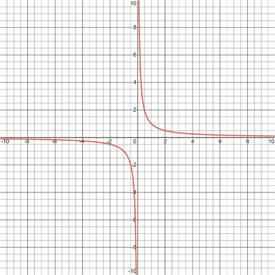
\includegraphics[width=]{"D:/Projects/latek/desmos-graph.png"}
    \caption{desmos-graph}
    \label{fig:graph1}
\end{figure}